% Created 2012-08-28 Tue 11:43
\documentclass[11pt]{article}
\usepackage[utf8]{inputenc}
\usepackage[T1]{fontenc}
\usepackage{graphicx}
\usepackage{longtable}
\usepackage{float}
\usepackage{wrapfig}
\usepackage{soul}
\usepackage{amssymb}
\usepackage{hyperref}


\title{B-Translator as a Software Engineering Project}
\author{Dashamir Hoxha}
\date{28 August 2012}

\begin{document}

\maketitle

\setcounter{tocdepth}{3}
\tableofcontents
\vspace*{1cm}


  The project B-Translator will be presented, trying to illustrate
  through it some software development/engineering concepts and
  practices (how they are actually applied in this project).


\section{Introduction}
\label{sec-1}


  Software Engineering is an interdisciplinary branch between
  programing and project management, that tries to make efficient and
  effective the process of developing new software, by identifying and
  trying to use principles and practices that have proved to be
  successful on the past projects. It was born as a response to the
  failures in software projects for a long time.

  Programing is an art, and so is the project management. As a result
  software engineering cannot be an exact discipline, although the
  word `engineering' seems to imply a set of well defined steps and
  rules. However, some guiding principles can be useful when applied
  wisely to the current situation. Anyway, the most important factor
  still remains the experience: you are good at managing software
  projects if you have enough experience with doing it.

  There are several models (or methods, or approaches, or paradigms)
  for managing a software project. The simples (and oldest) one is the
  waterfall model. The basic steps of the waterfall model are these:
\begin{itemize}
\item requirements
\item analysis
\item design
\item implementation
\item testing
\item deployment
\item maintenance
\end{itemize}
  These steps should be performed in the life cycle of every software
  development project. However the waterfall model is not very
  realistic, because in practice is very difficult to get everything
  right with the first attempt. For example while gathering the
  software requirement, most probably we can miss something; or maybe
  later there can be a request for updating the requirements.

  A better approach is the Iterative and Incremental model. The basic
  steps are the same, however the development is performed in several
  cycles, with each of these steps performed in almost each
  cycle. During the cycles the software is improved from an initial
  prototype to a full featured product.

  There are other methodologies and variations as well, like Agile
  Software Development, Extreme Programing, etc. However the bottom
  line remains that the best method to use depends on the concrete
  software that is to be developed, and any method that can be used
  should be adopted to match the current case.

  Therefore, here I will describe what I have done on the project
  B-Translator, trying to identify the principles and practices of
  Software Engineering that are used, instead of trying to fit this
  project to one of the standard approaches.


\section{Conception of the software}
\label{sec-2}


  Before a software starts to be built, the idea of such a software
  has to come somehow to mind. The idea for building such a software
  usually comes to mind because there is some problem to be solved, or
  some need to be fulfilled, which for some reasons, cannot be done
  (or cannot be done properly) by the existing software. Before
  anything else, a software engineer/developer should have a clear
  idea of the problem (or problems) that the software is trying to
  solve, and the overall aim (or goal) or the software.

\subsection{The problems that B-Translator tries to solve and its goals}
\label{sec-2.1}


   First of all, B-Translator is a software that helps to get feedback
   about l10n (localization, translations of programs into other
   languages). It also helps to unify all the different translations
   and to ensure consistency among the translations. It is intended to
   be used for the translations of programs into Albanian, but it can
   be used for any other languages as well.

   The motivation for developing such a software is that the
   traditional (current) l10n work-flow requires highly dedicated
   people, and does not allow (or at least does not facilitate) small
   contributions from random people that do not have such a high
   dedication, determination and enough free time.

   Also, the process of reviewing and correcting translations is not
   easy and does not facilitate the feedback from the users of the
   translated programs. Although the translators are usually very good
   and professional, they can make mistakes too, and sometimes they
   may miss the best translation for some certain terms. Some feedback
   from the crowd of the users would be more than welcome, if there
   are tools to collect and facilitate it.

   Another problem with translations is that sometimes they are not
   consistent. The same string has different translations in different
   programs, and sometimes even the same translator may have provided
   different translations for the same string in different cases. This
   happens mainly because each program/project has its own
   translations and there is no central repository for all the
   translations.

   To summarize, the goals of this software are these:
\begin{itemize}
\item Getting feedback about the translations from a wide crowd of
     people and users. This feedback can be in terms of votes for the
     best translation (when there are more than one translations for
     the same string), or it can be a new alternative translation (for
     an existing translation), or it can be a new translation
     suggestion (for a string that is not translated yet).
\item Helping to ensure consistency among the translations.
\item Merging translations from different sources (for example
     translations made on Launchpad and those made on KDE or GNOME).
\end{itemize}
\subsection{Are there any existing alternatives to B-Translator?}
\label{sec-2.2}


   To my knowledge, there are no such existing tools.  People
   frequently ask how B-Translator is different from Pootle.  Pootle,
   as far as I know, is just an online PO file editor; it doesn't have
   any features for collecting feedback from a crowd of people that
   are not translators.

\subsection{The meaning of B-Translator}
\label{sec-2.3}


   The name of the software is not the most important thing, however
   it should be somehow related to the basic idea of the software and
   to its goals, and it should be different from any other software.
   And of course it is better to be a nice name, rather than an ugly
   one.

   The codename \textbf{B-Translator} can be decoded like \textbf{Bee Translator},
   since it aims at collecting very small translation contributions
   from a wide crowd of people and to dilute them into something
   useful.

   It can also be decoded like \textbf{Be Translator}, as an invitation to
   anybody to give his small contribution for translating programs or
   making their translations better.


\section{Description of its features and functionality}
\label{sec-3}


  After having a clear idea of the overall aim and goals of the
  software, the software engineer should go into details about the
  features that the software should have and how it should work, so
  that it can properly achieve its goals. This is mainly a description
  of what the software should do and how it should do it, preferably
  in a simple language that even non-technical people (non-developers)
  can understand.

  Maybe we cannot get everything 100\% correct right from the
  beginning, however this approach is much better than starting to
  code right away, having just some vague ideas of what we are trying
  to build. Of course, we will take the chance later to correct and
  improve the feature requirements, as things become more clear.

\subsection{The features of B-Translator}
\label{sec-3.1}


   Here is a description of the main desired features of B-Translator.

\subsubsection{Open access}
\label{sec-3.1.1}


    Everybody should be able to use the system for the purpose of
    getting translation suggestions for a certain string, even
    unauthenticated (anonymous/guest) users.  Furthermore, it should
    be possible to use an API (web services), so that these
    suggestions can be retrieved and used even by external
    applications.

\subsubsection{Authenticated voting}
\label{sec-3.1.2}


    Submitting votes or new suggestions will be allowed only for the
    subscribed users (which have agreed to help and contribute). No
    contributions from anonymous/guests will be accepted.

\subsubsection{Tracking votes}
\label{sec-3.1.3}


    Votes and suggestions will not be anonymous. For each vote or
    suggestion, the user who submitted it will be recorded and
    saved. This will allow the user to see all the strings that he has
    already voted for, and also to change any of the votes, if he
    later changed his mind. At the same time it will prevent multiple
    votes by the same user for the same translation.

\subsubsection{Highly customizable}
\label{sec-3.1.4}


    The system should have a flexible configuration and customization
    page. This means that the user should be able to customize how much
    he would like to help and contribute. For example:
\begin{itemize}
\item how many translation votes per day (an upper limit)
\item which communication means he prefers (email, facebook,
       google+, twitter, website, android app, iPhone app, etc.)
\item which projects or packages he would like to focus on (for
       example, if the user selects the package KDE, only strings that
       belong to a project on this package will be sent to him for
       review and feedback)
\item which languages he would like to use as primary and secondary
       source languages (for example a user that is not confident in
       English, may choose to use French as a primary language and
       Italian+Spanish as secondary/helper languages)
\item sequential or random selection of strings (random is the
       default, but if the user is interested in just one or a few
       projects, he may prefer to review the strings sequentially)
\end{itemize}
\subsubsection{Evaluation algorithms}
\label{sec-3.1.5}


    The contribution and performance of the users should be measured
    and evaluated using certain algorithms and/or heuristics. The
    users will be awarded points based on their performance. Probably
    some rewarding mechanisms can be integrated later for the top
    contributors.

\subsubsection{Detailed and comprehensive reporting and statistics}
\label{sec-3.1.6}


    Different kinds of reports and statistics related to users,
    projects, activity etc. should be supported and provided.

\subsubsection{Integration with the existing workflow of the project translations}
\label{sec-3.1.7}


    Project translators will continue to work with their preferred
    tools (like Pootle, Lokalize, etc.). They will also continue to
    use their preferred workflows (the way that they coordinate their
    translation work with each-other and with the project releases).

    This system should help them to get feedback and possibly any new
    suggestions or translations from a big crowd of the
    contributors. The system should provide means and tools for easy
    integration with the workflow of the project translations.

    For example, it should allow the translation maintainers to import
    their existing translation files (PO files), and to export
    translation files that contain the most voted translations, as
    well as new suggestions (for translated strings) or new
    translations (for untranslated strings). It should also allow them
    to get the latest changes (suggestions, translations, etc.) since
    the last time that they checked, or since a predefined moment in
    the past.

    The latest changes should be exported in a format that is easy to
    review, modify and apply (diff or ediff).

    

\section{Analyzing the functionality in more details}
\label{sec-4}


  In the previous sections we discussed defining the aim and scope of
  the software (conception) and describing the desired features and
  functionality in general terms. Both of these steps belong to the
  phase called \textbf{defining requirements of the software}. The next step
  (or phase) is to analyze in more details how the software is
  supposed to work, and it is called \textbf{analysis} (or \textbf{functional   analysis}).

  Functional analysis is usually performed by identifying the \textbf{actors}
  (users or other programs/components that are interacting with our
  software/system), by identifying \textbf{use cases} (all the different
  cases when the actors need to interact with our software/system),
  and describing each \textbf{use case} (the details of how each interaction
  is done).

  In order to be clear and concise in describing such things, diagrams
  are often useful. The standard for drawing diagrams in software
  engineering domain is UML (Unified Modeling Language).

\subsection{The actors and use-cases of B-Translator}
\label{sec-4.1}


   The actors and use-cases that can be identified for B-Translator
   are these:
   
\begin{itemize}
\item \textbf{guest} (anonymous user)

\begin{itemize}
\item \textbf{get} translation suggestions for a string
\item \textbf{search} strings and translations
\item \textbf{export} translations
\item \textbf{comment} on translations
\end{itemize}

\item \textbf{contributor} (authenticated user)

\begin{itemize}
\item all the use-cases of guest
\item customize his own \textbf{preferences} and settings
\item \textbf{vote} (or \textbf{like}) translations
\item \textbf{suggest} new translations
\item \textbf{flag} inappropriate comments or translations
\item check his own contribution details in a \textbf{dashboard}, and how it
       compares with the others
\end{itemize}

\item \textbf{translator}

\begin{itemize}
\item all the use-cases of contributor
\item \textbf{import} translation files
\item \textbf{export} translations and suggestions
\end{itemize}

\item \textbf{moderator}

\begin{itemize}
\item all the use-cases of contributor
\item access \textbf{statistics} and other details
\item \textbf{resolve} flagged comments and translations
\end{itemize}

\item \textbf{administrator}

\begin{itemize}
\item manage overall software \textbf{configuration}
\item manage user access rights and \textbf{permissions}
\end{itemize}

\item \textbf{script}

\begin{itemize}
\item \textbf{update} translation data with the latest versions
\item \textbf{notify} users about relevant issues
\item apply suggested translations \textbf{upstream}, wherever possible and
       suitable
\end{itemize}

\item \textbf{peer} B-Translator installation

\begin{itemize}
\item request \textbf{sync} data (in case there are several B-Translation
       installations, they should be able to synchronize the data with
       each-other, if needed)
\end{itemize}

\end{itemize}
   These actors and use-cases are also presented in the following
   diagram (which is drawn using \href{http://www.umlet.com/}{Umlet}):
   \begin{figure}[htb]
\centering
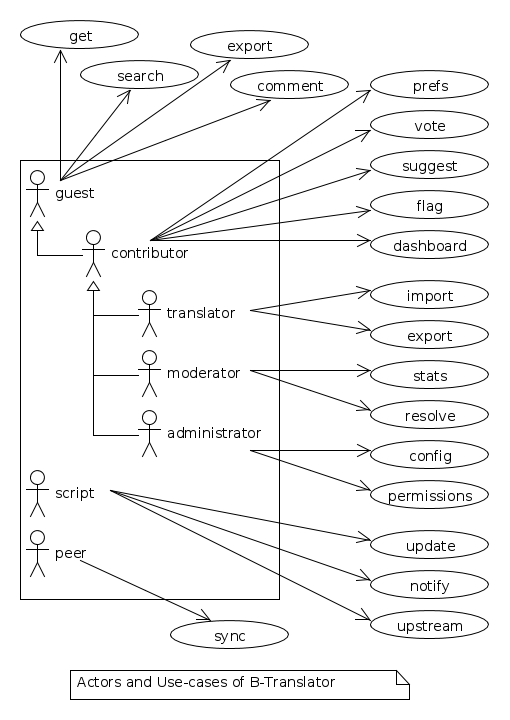
\includegraphics[width=13cm]{./uml/functional_analysis.png}
\caption{\label{fig:functional_analysis}Actors and Use-cases of B-Translator.}
\end{figure}

   There are also the cases when the software is accessed through a
   third party application (for example a Facebook, LinkedIn, Google+,
   Android, iPhone, or desktop application), through a web-service
   API, however these use-cases can be reduced to either the \textbf{guest}
   or \textbf{contributor} cases.

   I am not going to describe the details of each use-case because it
   would take lots of space. Anyway, most of them are almost obvious.

\subsection{Interfaces}
\label{sec-4.2}


\subsubsection{Suggestion interface}
\label{sec-4.2.1}


    This is the form where the (authenticated) user is presented with
    an English string and several translation suggestions for it, and
    he votes the one that he thinks is the best, or provides another
    suggestion which he thinks is better.

    The string to be translated is selected randomly, unless the user
    has selected `sequential' on his settings. The selection of the
    string is also done so that it complies with the restrictions
    imposed by the user on his settings (for example only from a
    certain project).

    The selection of the string should be also influenced by certain
    algorithms and heuristics, which should try to give more exposure
    to the strings that need more votes. For example if a string
    already got 10 votes and another one got just 2 votes, the second
    one should be more likely to be selected.

    This interface should be able to integrate somehow with facebook,
    email, google+, etc.


\subsubsection{Query interface}
\label{sec-4.2.2}


    On this form anybody (registered user or anonymous) can supply a
    string in English, and the system will return the translation
    suggestions related to it and the corresponding votes that each
    suggestion has.

    If the English string does not have an exact match on the DB, a
    list of similar strings will be returned and the user will choose
    to check one of them.

    This functionality of querying suggestions will be offered also by
    a web service so that it can be used by any external programs.


\subsubsection{User configuration interface}
\label{sec-4.2.3}


    Here the user customizes his settings, as described in the
    functional requirements.  Some of the things that he can customize
    are:
\begin{itemize}
\item how many translation reviews per day (default one)
\item which communication means he prefers (email, facebook, google+,
       twitter, website, android app, iPhone app, etc.)
\item which projects or packages he would like to focus on (for
       example, if the user selects the package KDE, only strings that
       belong to a project on this package will be sent to him for
       review and feedback)
\item which languages he would like to use as primary and secondary
       source languages (for example a user that is not confident in
       English, may choose to use French as a primary language and
       Italian+Spanish as secondary/helper languages)
\item sequential or random selection of strings (random is the
       default, but if the user is interested in just one or a few
       projects, he may prefer to review the strings sequentially)
\end{itemize}
\subsubsection{Export and import interfaces}
\label{sec-4.2.4}


    Usually everybody can export PO files, but only the users with
    certain permissions can import.


\subsubsection{Admin interfaces}
\label{sec-4.2.5}


    The admin should be able to customize the overall behavior of the
    module, to check activity, to get reports and statistics, to
    maintain the data (backup, restore, update) etc.
    

\section{Designing the software}
\label{sec-5}


  Design is a description in logical (abstract) terms of the parts and
  components that will make up the software, how they are composed,
  how they interact with each-other, etc. The UML diagrams can be
  useful again for describing concisely and clearly the entities,
  their relationships and interactions.  It is the last layer of
  abstract description, before the implementation (coding) of the
  software starts. However frequently there is not a clear distinction
  line between analysis and design, and between design and
  implementation.

  The design usually describes the database entities and
  relationships, the interfaces of the application, APIs (Application
  Programing Interfaces), classes and objects and their relationships,
  the most important processes and algorithms, etc. A good design
  should try to capture only the most important things, leaving out
  the obvious or unimportant things.

\subsection{The DB schema of B-Translator}
\label{sec-5.1}


   The DB tables and their fields:

\begin{description}
\item [Files] A PO file that is imported and can be exported from the
              DB.

\begin{description}
\item [fid : serial] Auto-increment internal identifier.
\item [filename : varchar(250)] The path and filename of the
          imported PO file.
\item [hash : char(40)] The SHA1() hash of the whole file content.
\item [potid : int] Reference to the template (POT) for which this
          PO file is a translation.
\item [lng : varchar(10)] The code of the translation language.
\item [headers : text] Headers of the imported PO file, as a long
          line. Needed mainly for exporting.
\item [comments : text] Translator comments of the file (above the
          header entry). Needed mainly for exporting.
\item [uid : int] Id of the user that imported the file.
\item [time : datetime] The date and time that the record was
          registered.
\end{description}

\item [Templates] POT files that are imported.

\begin{description}
\item [potid : serial] Auto-increment internal identifier.
\item [tplname : varchar(50)] The name of the POT template (to
          distinguish it from the other templates of the same
          project).
\item [filename : varchar(250)] The path and name of the imported
          POT file.
\item [pguid : char(40)] Reference to the project to which this PO
          template belongs.  it come from).
\item [uid : int(11)] Id of the user that registered the project.
\item [time : datetime] The date and time that the template was
          imported.
\end{description}

\item [Projects] A project is the software/application which is
                 translated by the PO files.

\begin{description}
\item [pguid : char(40)] Project Globally Unique ID, pguid =
          SHA1(CONCAT(origin,project))
\item [project : varchar(100)] Project name (with the release
          appended if needed).
\item [origin : varchar(100)] The origin of the project (where does
          it come from).
\item [uid : int(11)] Id of the user that registered the project.
\item [time : datetime] The date and time that the project was
          registered.
\end{description}

\item [Locations] Locations (lines) where a l10n string is found.

\begin{description}
\item [lid : serial] Internal numeric identifier of a line.
\item [sguid : char(40)] Reference to the id of the l10n string
          contained in this line.
\item [potid : int] Reference to the id of the template (POT) that
          contains this line.
\item [translator\_{}comments : varchar(500)] Translator comments in
          the PO entry (starting with ``\# ``).
\item [extracted\_{}comments : varchar(500)] Extracted comments in the
          PO entry (starting with ``\#. ``).
\item [line\_{}references : varchar(500)] Line numbers where the sting
          occurs (starting with ``\#: ``).
\item [flags : varchar(100)] Flags of the PO entry (starting with
          ``\#, ``).
\item [previous\_{}msgctxt : varchar(500)] Previous msgctxt in the PO
          entry (starting with ``\#| msgctxt ``).
\item [previous\_{}msgid : varchar(500)] Previous msgid in the PO entry
          (starting with ``\#| msgid ``).
\item [previous\_{}msgid\_{}plural : varchar(500)] Previous msgid\_{}plural
          in the PO entry (starting with ``\#| msgid\_{}plural ``).
\end{description}

\item [Strings] Translatable strings that are extracted from projects.

\begin{description}
\item [string : text] The string to be translated:
          CONCAT(msgid,CHAR(0),msgid\_{}plural)
\item [context : varchar(500)] The string context (msgctxt of the PO
          entry).
\item [sguid : char(40)] Globally Unique ID of the string, as hash
          of the string and context: SHA1(CONCAT(string,context))
\item [uid : int] ID of the user that inserted this string
          on the DB.
\item [time : datetime] The time that this string was
          entered on the DB.
\item [count : int/tiny] How often this string is encountered in
          all the projects. Can be useful for any heuristics that try
          to find out which strings should be translated first.
\item [active : boolean] The active/deleted status of the record.
\end{description}

\item [Translations] Translations/suggestions of the l10n strings.
          For each string there can be translations for different
          languages, and more than one translation for each language.

\begin{description}
\item [sguid : int] Reference to the id of the l10n string that is
          translated.
\item [lng : varchar(5)] Language code (en, fr, sq\_{}AL, etc.)
\item [translation : varchar(1000)] The (suggested) translation of
          the string.
\item [tguid : char(40)] Globally Unique ID of the translation,
          defined as the hash: SHA1(CONCAT(translation,lng,sguid))
\item [count : int/tiny] Count of votes received so far. This can be
          counted on the table Votes, but for convenience is stored
          here as well.
\item [uid : int] id of the user that initially suggested/submitted
          this translation
\item [time : datetime] Time that the translation was
          entered into the database.
\item [active : boolean] The active or deleted status of the record.
\end{description}

\item [Votes] Votes for each translation/suggestion.

\begin{description}
\item [vid : serial] Internal numeric identifier for a vote.
\item [tguid : char(40)] Reference to the id of the translation
          which is voted.
\item [uid : int] Reference to the id of the user that submitted the
          vote.
\item [time : datetime] Timestamp of the voting time.
\item [active : boolean] The active or deleted status of the record.
\end{description}

\item [Users] Users that contribute translations/suggestions/votes.

\begin{description}
\item [uid : int] The numeric identifier of the user.
\item [points : int] Number of points rewarded for his activity.
\item [config : varchar(250)] Serialized configuration variables.
\end{description}

\item [Snapshots] Snapshots are tgz archives of project-lng
                  translation files.

\begin{description}
\item [pguid : char(40)] Reference to the project.
\item [lng : varchar(10)] The language of translation.
\item [snapshot : mediumblob] The content of the tgz archive.
\item [uid : int] Id of the user that updated the snapshot for the
                    last time.
\item [time : datetime] The time of last update.
\end{description}

\item [Diffs] Diffs between the current state and the last snapshot.

\begin{description}
\item [pguid : char(40)] Reference to the project.
\item [lng : varchar(10)] The language of translation.
\item [nr : smallint] Incremental number of the diffs of a
                        project-language.
\item [diff : text] The content of the unified diff (diff -u).
\item [ediff : text] The embedded diff (generated with the command
                       poediff of pology).
\item [comment : varchar(200)] Comment/description of the diff.
\item [uid : int] Id of the user that inserted the diff.
\item [time : datetime] The date and time that the diff was saved.
\end{description}

\end{description}
   Files, Templates, Locations and Projects are related to the
   import/export of the PO files.  Snapshots and Diffs are used to
   export/extract the suggestions .  Projects and Categories can be
   used to limit the scope of the search (and other operations).

   A project contains the translations of a certain application
   (software).  A project can have several template (POT) files. A
   template file can have several PO files (one for each different
   language). Each of these PO files has many PO entries, which are
   stored in the table Locations.

   The table Locations stores only the comments, line references,
   flags, previous strings, etc. of each PO entry.

   The msgid (and msgctxt) of the entry is stored on the table
   Strings. A string can be connected to several locations, since the
   same string can be used on different projects.

   Each string can have several translations (or suggestions) in each
   language. Each translation can have many votes. Each vote is given
   by a certain user.

   \begin{figure}[htb]
\centering
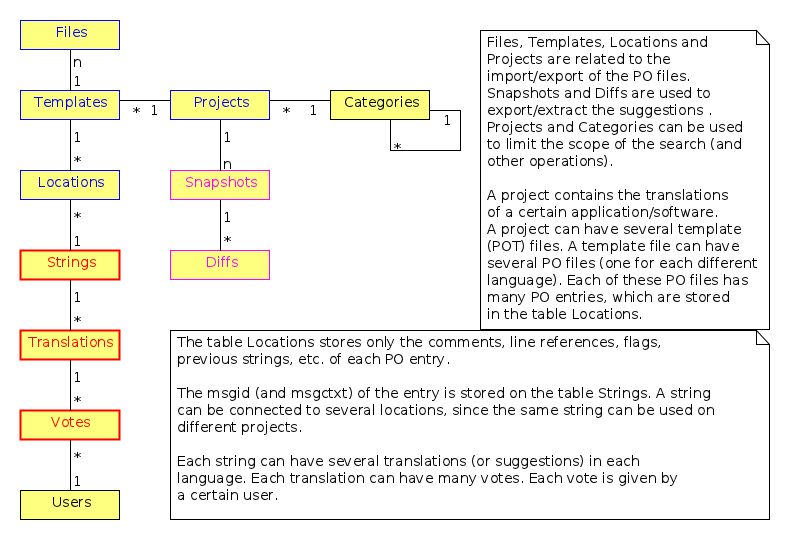
\includegraphics[width=13cm]{./uml/db_diagram.png}
\caption{\label{fig:db_diagram}Tables and their relations.}
\end{figure}

   \begin{figure}[htb]
\centering
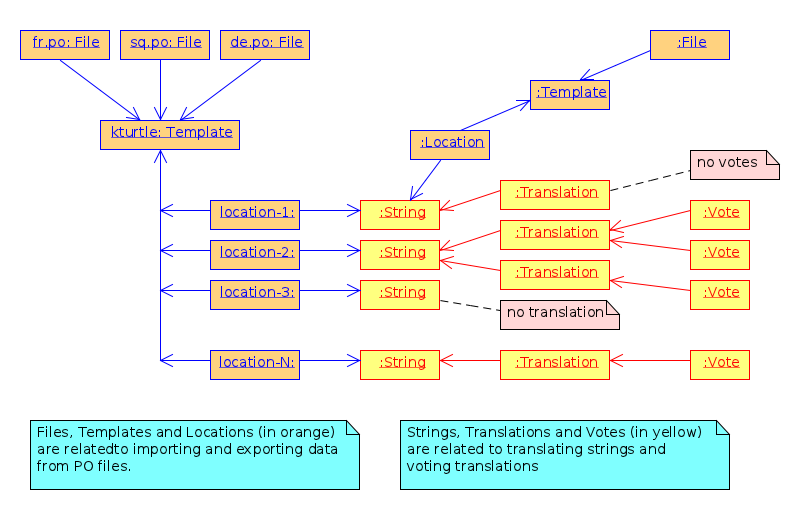
\includegraphics[width=13cm]{./uml/object_diagram_1.png}
\caption{\label{fig:object_diagram_1}Structure of the DB.}
\end{figure}

   \begin{figure}[htb]
\centering
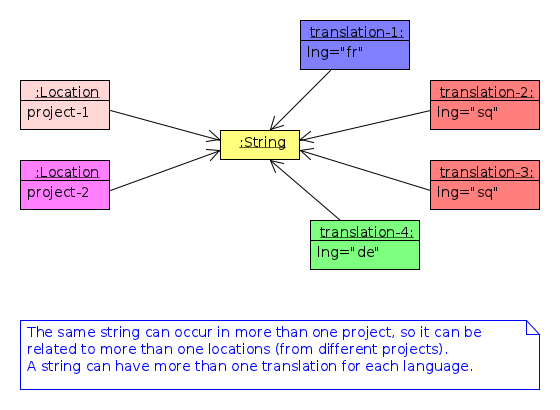
\includegraphics[width=12cm]{./uml/object_diagram_2.png}
\caption{\label{fig:object_diagram_2}Structure of the DB.}
\end{figure}

   \begin{figure}[htb]
\centering
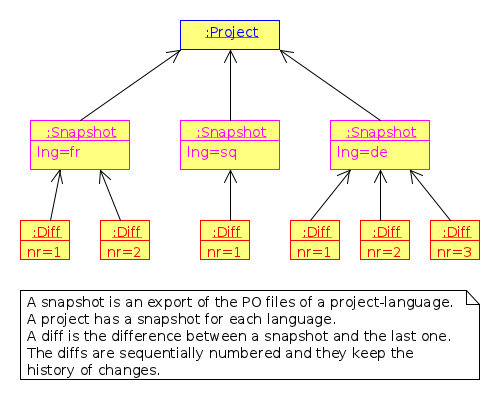
\includegraphics[width=12cm]{./uml/object_diagram_3.png}
\caption{\label{fig:object_diagram_3}Structure of the DB.}
\end{figure}


\subsection{API}
\label{sec-5.2}



\section{Construction (implementation/development)}
\label{sec-6}


  Implementation is the process of actually building the software.
  Before the implementation starts, several decisions have to be done, like:
\begin{itemize}
\item what platform to use
\item what programing language or framework should be used
\item what database should be used
\item what tools to use for development
\item how to coordinate the work of several developers
\item programing standards to be used
\item etc.
\end{itemize}
  For B-Translator it was obvious that it was going to be a web
  application, running on a LAMP platform (Linux+Apache+MySQL+PHP).
  Moreover, I decided to implement it as a Drupal module, in order to
  take advantage of the other existing Drupal modules. Drupal is a
  powerful framework for building web application, it has a powerful
  API, and there are lots of available modules that implement various
  features. This way I could focus on building only the functionality
  that is specific for my problem, and use the available modules for
  building a fully functional web application. Furthermore, I decided
  to use Drupal7, since that was the latest version of Drupal when I
  started, although the support of the additional modules was not so
  good at that time.

  For programing and development I use the Emacs editor, which is
  quite powerful. Also this is the editor that I am most familiar
  with, and I always use it for my programing tasks.

  As a version control system I use git. Actually the repository of
  the project is hosted on github.com
  (\href{https://github.com/B-Translator/server}{https://github.com/B-Translator/server}). Usage of a version control
  system is a must for every software development project, because:
\begin{itemize}
\item It keeps all the history of changes in the project and allows you
    to roll back to a previous state, in case that something goes
    wrong.
\item It allows you to have tags and branches, which help the management
    of the development process.
\item It allows several developers to easily coordinate and merge their
    work with each other.
\item It simplifies the task of providing patches for external
    contributors.
\end{itemize}
  The coding style and standards of B-Translator are those used by
  Drupal.  For unit testing and functional testing the module
  `simpletest' of Drupal is used. It works by defining several test
  cases, and then making sure that the module passes successfully all
  of them.

  For communication/discussions among the developers there is an IRC
  chatroom named \textbf{\#btranslator} on \textbf{irc.freenode.net}. There is also
  the group/forum/mailing-list \href{https://groups.google.com/forum/?hl=en&fromgroups#!categories/btranslator}{B-Translator} on Google, for
  notifications, discussions, etc. There is as well the channel
  \textbf{@btranslator} on Twitter, mostly for notifications.

  Actually, right now I am the only developer of the project, however
  I do hope that in the future there will be other developers and
  contributors as well. If you are interested to help, please contact
  me (at dashohoxha@gmail.com) or join the forum above.


\section{Managing the project}
\label{sec-7}


  Software engineering is not just about programing or development,
  but it is also about project management. Project management includes
  making a plan about how we are going to build the software, defining
  the things or tasks that need to be done, breaking down the tasks
  into smaller ones, assigning importance or priorities to the tasks,
  deciding which ones should be done earlier and which ones can be
  done later, defining milestones and grouping tasks to them
  (according to the time that they should be completed), assigning
  tasks to people, etc.

  The majority of tasks usually are related to programing and
  implementation, however anything else can be a task (for example,
  collecting requirements, performing the functional analysis, etc.).
  
  There are some steps or phases that are common for all software
  engineering projects, like:
\begin{itemize}
\item collecting/updating the requirements
\item defining/refining features and functionality
\item analyzing/understanding/describing the details of each feature
\item making/correcting design decisions
\item implementing or improving features
\item testing, debugging and making sure that they work correctly
\item etc.
\end{itemize}
  
  How these phases are combined together depends on the software that
  is to be build. If you have enough experience with building such
  kind of software, and you have a clear idea from the beginning about
  what is to be built, then a waterfall approach might be OK.

  However, in most cases things are not very clear right from the
  beginning, and they become more clear as you work on the project, do
  some implementation and testing, get feedback from the users,
  etc. This is especially true if the software that you are trying to
  build is kind of innovative, something that nobody else has tried to
  build before. In this case an `iterative and incremental' model could
  be more suitable. In this model you build and release an initial
  product (or prototype), and with the experience collected during the
  process and any feedback from the users, start again from the
  beginning and refine the requirements, analysis etc. and build
  another release of the software. These cycles can be repeated as
  many times as necessary, and in each cycle incremental
  changes/improvements are made to the software.

  B-Translator has followed an iterative and incremental life cycle.
  Although from the previous sections it may appear that things
  happened in a clean waterfall model, the truth is that the current
  requirements, functional analysis, design, etc. are the result of
  several iterations (cycles). For example:
\begin{itemize}
\item The design of the database became more clear only after starting
    to implement it. Actually I had to change the structure of the
    database several times, until it was suitable.
\item Initially I depended on importing the data collected by
    \href{http://open-tran.eu/}{open-tran.eu}. However, I decided later to implement my own scripts
    for getting translation files and importing them on the DB.
\item Integration with the existing workflow of the project translations
    was something that occurred to me later, after I had started
    implementation.
\item Integration required the ability to import and export PO files,
    and this made me add some extra tables for keeping the relevant
    information.
\item Initially I did not think about the possibility of exporting diff
    (and ediff) files.  After deciding to implement such a feature, I
    had to add a few more tables in the design of the database.
\item The possibility for appending comments to each translation was
    suggested to me by one of the translators.
\end{itemize}
  The tool that I use for keeping the project organized is the
  \href{http://orgmode.org/}{mode-org of Emacs}. It is a wonderful tool, simple and flexible, but
  has also advanced features if you need them. It can be used for
  keeping notes, for task management, and also for documentation
  writing (all the documents related to B-Translator, including this
  one, are composed with it). Its wiki-like syntax, combined with the
  power of Emacs, make it very practical.

  Right now, for bug reporting, feature requests, etc. the issues
  section on GitHub can be used:
  \href{https://github.com/B-Translator/server/issues}{https://github.com/B-Translator/server/issues} . Later maybe I
  can install \href{http://trac.edgewall.org/}{trac}, which is nice tool for software project
  management.


\section{Documentation}
\label{sec-8}


  Documentation describes how to install the software, how it works,
  how it should be used, etc.

\subsection{Installation of B-Translator}
\label{sec-8.1}


   A full distro including Drupal core (with patches) and the
   \emph{btranslation} installation profile can be built like this:

\begin{verbatim}
cd /var/www/
sudo git clone https://github.com/B-Translator/server.git
sudo B-Translator/install/all.sh
\end{verbatim}



   For more detailed information about installation see:
   \href{https://github.com/B-Translator/server/blob/master/docs/INSTALL.org}{https://github.com/B-Translator/server/blob/master/docs/INSTALL.org}

\subsection{How B-Translator works}
\label{sec-8.2}


\subsubsection{Build a dictionary of l10n strings}
\label{sec-8.2.1}


    The source of the translation data used by the software are the
    POT/PO files of the projects.  The PO template files (POT) contain
    the list of translatable strings of a project (in English), and the
    PO translation files contain the strings and the corresponding
    translations for a certain language.  (More information and details
    about PO/POT formats and the translation process is provided by
    `info gettext`.)

    These PO files are imported into the DB of the software. This
    import creates a dictionary of strings and their corresponding
    translations. The same string can be used in more than one
    projects, but in the dictionary it is stored only once. However, if
    the same string has different translations in several projects, all
    of the distinct translations will be stored into the DB.

\subsubsection{Collect feedback from users/reviewers}
\label{sec-8.2.2}


    These strings and the corresponding translations are presented for
    review to a large community of reviewers/users. The reviewers
    indicate which translation they think is the best by voting for it.
    They can also suggest any new translations (or suggest translations
    for strings that are yet un-translated). These new translations and
    the votes/likes of the reviewers are stored in the DB as well

    The review process happens slowly and gradually during a long
    time. We can assume that each reviewer checks only one string each
    day, and that there is a very large number of reviewers that give
    feedback each day. The feedback can be collected through different
    channels, like web interface, social networks (Facebook,
    Google+, Twitter), email, mobile apps, etc.

\subsubsection{Export the revised translations}
\label{sec-8.2.3}


    Besides the dictionary of strings and translations, the import of
    PO files saves also the structure of these files and all the
    relevant data that are needed to export them again from the
    DB. However, during the export of the PO files, the most voted
    translations for each string are retrieved from the DB, instead of
    the original translations that were imported. This is how the
    input/feedback of the reviewers is transferred into the PO
    files. These exported PO files can then be uploaded/committed into
    the repositories of the corresponding projects.

\subsubsection{The process/workflow for a project without translation}
\label{sec-8.2.4}


    According to the steps described above, the process/workflow for a
    project that has no translation yet, would be like this:
\begin{enumerate}
\item Checkout POT files from the repository of the project.
\item Import them into the DB.
\item Over some time, collect translation suggestions from the users.
       These translations can also be reviewed and evaluated by other
       users.
\item Export the PO files from the DB.
\item Review, fix and reformat them as needed.
\item Upload/commit the PO files into the repository of the project.
\item When a new POT file is released, start over again from the
       beginning (but this time we also import the PO file, besides the
       POT file).
\end{enumerate}
    This process works well if there are no traditional translators to
    the project, and there is no other translation workflow happening
    concurrently (in parallel) with this one. Otherwise there would be
    a need to integrate these two workflows so that they don't override
    each-other.

\subsubsection{Exporting only the latest suggestions (diffs)}
\label{sec-8.2.5}


    In practice actually there is an existing translation workflow for
    almost all the projects. This translation is done either by using a
    Pootle system or by using PO editors. So, it is important that our
    workflow integrates with this existing workflow.

    This integration is helped by exporting diffs instead of exporting
    PO files. These diffs are retrieved by the maintainers of the
    existing translation workflow (translators), and they contain the
    latest translation suggestions made by the reviewers through the
    feedback system. Such diffs can then be easily checked by the
    translators, and if they find them appropriate they can apply them
    to the PO files on the existing workflow.

    Diffs are made between the current state of translations and the
    last snapshot of the translations. This ensures that diffs do not
    contain any suggestions that have been included already in the
    previous diffs, and so making more easy the work of the
    translators. The translator is usually interested only on the last
    diff, however the previous diffs are saved in the DB as well, in
    order to have a full history of the suggested translations over the
    time. Whenever a translator checks the latest diff, he should also
    make a snapshot, so that the translations that have been already
    suggested to him are not suggested again. Making a snapshot will
    also generate the diff with the previous snapshot and store this
    diff on the DB as well.

\subsubsection{The process/workflow for an integrated translation}
\label{sec-8.2.6}


    The process/workflow for the case when the feedback provided by the
    system is integrated in the mainstream translation workflow is like
    this:
\begin{enumerate}
\item Checkout the latest version of the POT and PO files from the
       repository of the project.
\item Import POT files and PO files into the DB.
\item Over some time, collect votes and new translation suggestions
       from the users.
\item Time after time (for example each month), the mainstream
       translator checks out the last diffs, containing the latest
       suggestions (and makes a snapshot as well).
\item The translator reviews the latest suggestions and applies them
       in the mainstream translation, if he finds them appropriate.
\item Periodically (for example once or twice a year) go back to steps
       (1) and (2) and import the POT and PO files again. This
       re-import may introduce new strings and translations, but will
       not affect the existing strings, translations and votes.
\end{enumerate}
\subsection{Drupal interfaces (paths)}
\label{sec-8.3}


\subsubsection{translations[/<lng>/<sguid>]}
\label{sec-8.3.1}


    This interface presents a string and its available translations to
    the user. The user will vote one of them as the best translation,
    or will provide a new translation that he thinks is better.

    <sguid> is the hash of the string that is being translated. If not
    given, then a random string will be selected.

    The original string is usually presented in English, but
    additional languages can be presented as well, if the user is not
    confident with English. (He can select these options on the user
    settings page as well.)


\subsubsection{translations/search?lng=..\&limit=..\&mode=..\&words=..}
\label{sec-8.3.2}


    Displays a list of strings and the corresponding suggestions, which
    match some filter conditions. Filter conditions can be modified on
    the interface. Search can be done by the content of the strings and
    suggestions, and can be limited in scope by the project, by the author
    of suggestions, by the submission date, etc.

    From the displayed list, it is also possible to view details (for
    string or suggestion), to submit votes, etc.


\subsubsection{translations/project}
\label{sec-8.3.3}

\begin{itemize}
\item translations/project/list ([/origin[/project[/format]]])
\item translations/project/export (/origin/project/language)
\item translations/project/export\_{}tgz (/origin/project/language)
\item translations/project/diff (/origin/project/lng[/nr[/ediff]])
      Return the diff/ediff of the PO files for a given
      origin/project/lng/nr.  If the parameter `nr' is `-', it returns
      the latest most-voted suggestions since the last snapshot.  If
      the parameter `nr' is missing, it returns a list of the saved
      diffs instead.
\end{itemize}
\subsubsection{translations/user\_{}settings}
\label{sec-8.3.4}

    The user can set:
\begin{itemize}
\item translation language
\item the preferred source language(s)
\item how many reviews per day is willing to make
\item etc.
\end{itemize}
\subsubsection{translations/admin}
\label{sec-8.3.5}

\begin{itemize}
\item translations/admin/config
\item translations/admin/dashboard
\item translations/admin/reports
\item translations/admin/stats
\end{itemize}
\subsection{Importing and exporting translation files}
\label{sec-8.4}


\subsubsection{Translation files}
\label{sec-8.4.1}


    The translation files that are imported into the DB are retrieved
    from the repository of the corresponding projects. This is done by
    the scripts in the directory \texttt{get/}, which checkout (or update)
    these files from each projects' repository.

    The way of getting these files is slightly different for different
    projects. However all of them are placed in the directory
    \texttt{\$data\_root}, which is defined in \texttt{config.sh}. Besides \texttt{\$data\_root},
    \texttt{config.sh} defines also the variable \texttt{\$languages}, which is a list
    of the codes of the languages that are supported by the system.
    
    Projects on the \texttt{\$data\_root} are also grouped (categorized) by
    origin.  For example all the GNOME projects are placed on the same
    directory, all the KDE projects on another directory, and so on.
    Under the `origin' directory, there is a subdirectory for each
    language, and under it usually there is a subdirectory for each
    project, containing all the translation files of the project, in
    any structure that is suitable for the project.

    Some projects have just a single translation (PO) file (for example
    those of GNOME or ubuntu), some others have several translation
    files (like those of KDE), and some others have many translation
    files (like those of LibreOffice and Mozilla).

    In the case of Mozilla, translation files are not in gettext format,
    so they are converted to PO files using \texttt{moz2po} (from Translation
    Toolkit).


\subsubsection{Importing}
\label{sec-8.4.2}


    Translation files are imported into the database by the scripts in
    the directory \texttt{import/}.

    Importing is done in two steps: the first step is to import the
    template (POT) files of the project, and the second step is to
    import the translation (PO) files for each language.  A POT file
    usually has a corresponding PO file for each language. 

    The template (POT) files contain the translatable strings of the
    project, with empty translations (this is why they are called
    templates). The translation (PO) files contain the same strings
    as the POT files, but with the corresponding translations for a
    certain language. In the import scripts, usually the French (fr)
    translation files are used as template files.

\begin{itemize}

\item Importing template files (pot\_{}import.php)\\
\label{sec-8.4.2.1}


     Template files are imported by \texttt{pot\_import.php}, which is called
     like this:

\begin{verbatim}
$ ./pot_import.php

Usage: ./pot_import.php origin project tplname file.pot
  origin   -- The origin of the project (ubuntu, GNOME, KDE, LibreOffice, etc.)
  project  -- The name of the project that is being imported.
  tplname  -- The name of the PO template.
  file.pot -- The POT file of the project.

Examples:
  ./pot_import.php KDE kdeedu kturtle test/kturtle.pot
  ./pot_import.php KDE kdeedu kturtle test/kturtle_fr.po
\end{verbatim}



     \texttt{pot\_import.php} creates a new template and a new project (if
     needed).  If the given \underline{origin+project} already exists, then the
     existing project is used.  However, if the given template already
     exists (for this project), then it is deleted first (along with the
     locations and files related to it), and then recreated.
      
     Along with the template, locations that are contained in this
     template are created as well. The string corresponding to each
     location is created only if it does not already exist. Otherwise
     the existing string is referenced instead (and the reference count
     of the string is incremented).


\item Importing translation files (po\_{}import.php)\\
\label{sec-8.4.2.2}


     Translation files are imported by \texttt{po\_import.php}, which is called
     like this:

\begin{verbatim}
$ ./po_import.php

Usage: ./po_import.php origin project tplname lng file.po
  origin  -- The origin of the project (ubuntu, GNOME, KDE, LibreOffice, etc.)
  project -- The name of the project.
  tplname -- The name of the PO template.
  lng     -- The language of translation (de, fr, sq, en_GB, etc.).
  file.po -- The PO file to be imported.

Example:
  ./po_import.php KDE kdeedu kturtle fr test/kturtle.po
\end{verbatim}



     \texttt{po\_import.php} imports a new PO (translation) file.  It assumes
     that the POT file of the project has already been imported,
     otherwise it will quit without doing anything.  If the file has
     been already imported, then it is skipped.
       
     For each file, all the information that is needed for exporting it
     is stored, like the file name and path, the headers of the file,
     the content of the file, etc.
       
     Along with the file, it also inserts the translations for the
     corresponding strings, when such translations do not exist.



\item Import example (pingus.sh)\\
\label{sec-8.4.2.3}


     The most simple example of importing a project is \texttt{pingus.sh}. The
     other scripts import many projects from the same origin at once,
     and have logic about getting the project name, finding the files,
     etc. Also, they may have several (or many) template files for each
     project, which makes the logic even more complex.

     The basic import code of \texttt{pingus.sh} is this:

\begin{verbatim}
### make last snapshots before re-import
make-last-snapshot $origin $project fr
make-last-snapshot $origin $project sq

### import the template
potemplate=pingus
./pot_import.php $origin $project $potemplate $po_dir/pingus-fr.po

### import the PO files
./po_import.php $origin $project $potemplate fr $po_dir/pingus-fr.po
./po_import.php $origin $project $potemplate sq $po_dir/pingus-sq.po

## make initial snapshots after (re)import
make-snapshot $origin $project fr $po_dir/pingus-fr.po
make-snapshot $origin $project sq $po_dir/pingus-sq.po
\end{verbatim}



     The main import code is: importing first the template, and then
     importing the translation file for each language. However, before
     the import we \emph{make a last snapshot} of the existing project, and
     after the import we also \emph{make a snapshot}. These two functions,
     \texttt{make-last-snapshot} and \texttt{make-snapshot} are defined on
     \texttt{make-snapshot.sh}, which is included in \texttt{pingus.sh}. They will be
     discussed in more details in the section about the snapshots and
     diffs.



\item Import scripts\\
\label{sec-8.4.2.4}


     The other scripts in the directory import are used to import
     projects from a certain origin. For example \texttt{kde.sh} imports (or
     re-imports) all the KDE projects, \texttt{office.sh} imports/re-imports
     all the LibreOffice projects, and so on.

     If a list of projects is passed on the command-line to these
     scripts, then only the specified projects will be imported (instead
     of all the projects.)


\end{itemize} % ends low level
\subsubsection{Exporting}
\label{sec-8.4.3}


    As we have seen, besides the strings and translations, the import of
    PO files saves also the structure of these files and all the
    relevant data that are needed to export them again from the DB.

    Export scripts are in the directory \texttt{export/}.

\begin{itemize}

\item Exporting PO files (po\_{}export.php)\\
\label{sec-8.4.3.1}


     The script \texttt{po\_export.php} is used to export a single PO file. It
     is used like this:

\begin{verbatim}
$ ./po_export.php

Usage: ./po_export.php origin project tplname lng [file.po [export_mode]]
  origin      -- the origin of the project (ubuntu, GNOME, KDE, etc.)
  project     -- the name of the project to be exported
  tplname     -- The name of the PO template.
  lng         -- translation to be exported (de, fr, sq, en_GB, etc.)
  file.po     -- output file (stdout if not given)
  export_mode -- 'most_voted' (default) or 'original'

The export mode 'most_voted' (which is the default one) exports the
most voted translations and suggestions.
The export mode 'original' exports the translations of the original
file that was imported (useful for making an initial snapshot of
the project).
If the export mode is not given as an argument, then the env variable
PO_EXPORT_MODE will be tried.

Examples:
  ./po_export.php KDE kdeedu kturtle fr > test/kturtle_fr.po
  ./po_export.php KDE kdeedu kturtle fr test/kturtle_fr.po original
\end{verbatim}



     The PO file to be exported is identified by \texttt{\{origin, project,      tplname, lng\}}.

     If the export mode is \emph{original}, then the same translations that
     were imported are exported again. This is useful for making initial
     snapshots and diffs, which we will discuss later. However it should
     be noted that the exported file is not exactly the same as the
     imported file.  One reason is that the formatting can be different,
     although the strings and translations are the same. Another reason
     is that during import some entries are skipped. like
     `translator-credits' etc.

     If the export mode is \emph{most\_{}voted}, and some of the translations
     have been voted, then the most voted translation is exported
     instead. This is how the input/feedback of the reviewers is
     transferred into the PO files. But since the formatting of the
     exported file is not exactly the same as the imported file, this
     exported file cannot be used directly to be committed to the project
     repository. Instead it is merged somehow with the existing PO file
     of the project. This merge can be simply done by \texttt{msgmerge}, or by
     tools like \texttt{lokalize} that facilitate merging of PO files. Another
     option is to get the differences between the exported file and the
     original file and to apply them to the current PO file.


\item Exporting projects (export.sh)\\
\label{sec-8.4.3.2}


     To export all the PO files of a project, the script \texttt{export.sh} is
     used:

\begin{verbatim}
$ ./export.sh
Usage: ./export.sh origin project lng output_dir
\end{verbatim}



     If \texttt{project==all}, then all the projects of the given origin will be
     exported. It the environments variable QUIET is defined, then it
     will be less verbose (will not output much progress/debug info).

     The exported files are saved under the directory \texttt{output\_dir}.
     Their path under the \texttt{output\_dir} is the same as the path of the
     imported files. This is useful for making diffs with the original
     files of the project.
    

\item Exporting projects in tgz format (export\_{}tgz.sh)\\
\label{sec-8.4.3.3}


     This script is usually called from the web (through the REST API)
     to export all the PO files of a project, in .tgz format.

\begin{verbatim}
$ ./export_tgz.sh
Usage: ./export_tgz.sh origin project lng [output_dir]
\end{verbatim}



     If project==all, then all the projects of the given origin will be
     exported. If the \texttt{output\_dir} is not given, then the \texttt{/tmp}
     directory will be used.

     It outputs the path of the created archive.


\end{itemize} % ends low level
\subsubsection{Snapshots and diffs}
\label{sec-8.4.4}


    A \emph{snapshot} is an export from the DB of the current PO files of a
    project-language. This export (which is a .tgz archive) is stored in
    the DB. A project has a snapshot for each language. Snapshots are
    useful for generating the \emph{diffs}.

    A \emph{diff} is the difference between the snapshot and the previous
    snapshot.  The diffs are stored in the DB as well. They are
    sequentially numbered and keep the history of changes.

    There are two types of diffs that are generated and stored. One is
    the \emph{unified diff} (\texttt{diff -u}) and the other the \emph{embedded diff}
    (generated by pology
    \href{http://websvn.kde.org/trunk/l10n-support/pology/}{http://websvn.kde.org/trunk/l10n-support/pology/})

    Diffs ensure that translators get only the latest feedback (since
    the last snapshot), without having to review again the suggestions
    made previously. So, they make easier the work of the translators.
    However the previous diffs are saved in the DB as well, in order to
    have a full history of the suggested translations over the time.


\begin{itemize}

\item Keeping diffs in the DB (db\_{}diff.php)\\
\label{sec-8.4.4.1}


     The script \texttt{db\_diff.php} is used to \emph{add}, \emph{list} or \emph{get} the diffs
     from the DB. It is just an interface to the DB.


\begin{verbatim}
$ ./db_diff.php

Usage: ./db_diff.php add  origin project lng file.diff file.ediff [comment [user_id]]
       ./db_diff.php list origin project lng
       ./db_diff.php get  origin project lng number (diff|ediff) [file]

  origin     -- the origin of the project (ubuntu, GNOME, KDE, etc.)
  project    -- the name of the project to be exported
  lng        -- language of translation (de, fr, sq, en_GB, etc.)
  file.diff  -- file in `diff -u` format
  file.ediff -- file in ediff (embedded diff) format
  comment    -- optional comment about the ediff file that is being added
  user_id    -- optional (drupal) uid of the user that is adding the ediff
  number     -- the number of ediff that is being retrieved

Examples:
  ./db_diff.php add LibreOffice sw fr LibreOffice-sw-fr.diff LibreOffice-sw-fr.ediff
  ./db_diff.php list LibreOffice sw fr
  ./db_diff.php get LibreOffice sw fr 5 diff > LibO/fr/sw_5.diff
  ./db_diff.php get LibreOffice sw fr 5 ediff > LibO/fr/sw_5.ediff
\end{verbatim}



     This script is usually called from other scripts (not directly from
     the command line).



\item Keeping snapshots in the DB (db\_{}snapshot.php)\\
\label{sec-8.4.4.2}


     The script \texttt{db\_snapshot.php} is used as a DB interface for the snapshots.


\begin{verbatim}
$ ./db_snapshot.php

Usage: ./db_snapshot.php (init|update|get) origin project lng file.tgz

  origin   -- the origin of the project (ubuntu, GNOME, KDE, etc.)
  project  -- the name of the project to be exported
  lng      -- language of translation (de, fr, sq, en_GB, etc.)
  file.tgz -- tgz archive of the snapshot of the project

The operation 'init' is used to insert into the DB the snapshot
for the first time. The operation 'update' to update it, and
'get' to retrive it from the DB.

Examples:
  ./db_snapshot.php init   LibreOffice sw fr LibreOffice-sw-fr.tgz
  ./db_snapshot.php update LibreOffice sw fr LibreOffice-sw-fr.tgz
  ./db_snapshot.php get    LibreOffice sw fr LibreOffice-sw-fr.tgz
\end{verbatim}



     The operation \texttt{init} will first delete a snapshot, if it already
     exists in the DB. This script is usually called from other scripts
     (not directly from the command line).


\item Making a diff (make\_{}diff.sh)\\
\label{sec-8.4.4.3}


     This script compares the current translation files of an \texttt{\{origin,      project, lng\}} with the last snapshot.
   

\begin{verbatim}
$ ./make_diff.sh

Usage: ./make_diff.sh origin project lng

Export the current state of translation files of a project-language
and make a diff with the last snapshot.
\end{verbatim}



     It does these:
\begin{enumerate}
\item Export the current files for the given \texttt{\{origin, project, lng\}}
        (by calling \texttt{export.sh})
\item Get the (last) snapshot for \texttt{\{origin, project, lng\}}
\item Make the difference between them with \texttt{diff -rubB} and with \texttt{pology}
\end{enumerate}
     When it is done, it leaves in its own directory the files
     \texttt{origin-project-lng.tgz} (which contains the exported files),
     \texttt{origin-project-lng.diff} and \texttt{origin-project-lng.ediff}.

    It outputs some debug information as well, but if the \texttt{QUIET}
    environment variable is define, this output is suppressed.



\item Making a snapshot (make\_{}snapshot.sh)\\
\label{sec-8.4.4.4}



\begin{verbatim}
$ ./make_snapshot.sh

Usage: ./make_snapshot.sh origin project lng [diff_comment]

Make the diff with the last snapshot and store it in DB.
Save in DB the current snapshot.
\end{verbatim}



     This script just calls \texttt{make\_diff.sh} and stores in DB the files
     \texttt{origin-project-lng.diff} and \texttt{origin-project-lng.ediff}, if they
     are not empty. It also updates the snapshot of \texttt{\{origin, project,      lng\}} with the file \texttt{origin-project-lng.tgz}. Finally it cleans all
     the three files generated by \texttt{make\_diff.sh}.

     \texttt{make\_diff.sh} is separated from \texttt{make\_snapshot.sh} because it
     needs to be used also by the REST API
     \texttt{translations/project/diff/origin/project/lng/-} to generate the
     changes (diffs) since the last snapshot.



\item Lifecycle of the diffs and snapshots\\
\label{sec-8.4.4.5}


     When a project is imported, an initial snapshot is created and
     stored in the DB as well. This initial snapshot contains the
     original files that were used for the import. It is done like this:

\begin{verbatim}
### store the tgz file into the DB as a snapshot
../export/db_snapshot.php init $origin $project $lng $snapshot_tgz
\end{verbatim}



     Immediately after the initial snapshot, another snapshot is done,
     by exporting files in the \emph{original} mode.

\begin{verbatim}
### make a second snapshot, which will generate a diff
### with the initial snapshot, and will save it into the DB
export PO_EXPORT_MODE='original'   ## set the export mode for po_export.php
diff_comment="Import diff. Contains formating changes, any skipped entries, etc."
../export/make_snapshot.sh $origin $project $lng "$diff_comment"
\end{verbatim}


     This snapshot will also generate a diff, which contains the
     differences that come as a result of formatting changes between the
     original format and the exported format. It also contains the
     entries that are skipped during the import.
     
     Whenever a translator checks the latest diff, he should also make a
     snapshot, which will also generate the diff with the previous
     snapshot (and store it on the DB). As a result, the translations
     that have been already suggested to him will not be suggested
     again.

     When the time comes to re-import a project, a last snapshot is made
     automatically before the import, in order to store as a diff any
     latest (unchecked) suggestions.

\begin{verbatim}
### make a last snapshot before the import (useful in the case of re-import)
export PO_EXPORT_MODE='most_voted'   ## set the export mode for po_export.php
diff_comment="Contains the latest suggestions before import."
../export/make_snapshot.sh $origin $project $lng "$diff_comment"
\end{verbatim}


   
     Then an initial snapshot is made again with the original files,
     using \texttt{db\_snapshot.php init ...} (which will not generate any
     diff).  After it, a snapshot using the \texttt{original} mode of export is
     made again, which will generate again any formatting changes and
     save them as a diff.

     However, in the case of re-import, another snapshot is needed,
     using the \texttt{most\_voted} mode of export, which will generate a diff
     that contains all the feedback and suggestions made before the
     re-import.

\begin{verbatim}
### make another snapshot, which will contain all the previous suggestions
### (before the import), in a single diff
export PO_EXPORT_MODE='most_voted'   ## set the export mode for po_export.php
diff_comment="Initial diff after import. Contains all the previous suggestions (before the last import)."
../export/make_snapshot.sh $origin $project $lng "$diff_comment"
\end{verbatim}


     Usually this diff contains the suggestions that the translator has
     already rejected, and making this snapshot ensures that they are
     not suggested again to him.

     This logic of the initial snapshots and diffs is applied by calling
     the functions \texttt{make-last-snapshot()} and \texttt{make-snapshot()}, which
     are defined on the file \texttt{import/make-snapshot.sh}. They are
     included and called automatically by the import scripts, before and
     after each import.


\item Getting diffs from the web (wget\_{}diff.sh)\\
\label{sec-8.4.4.6}


     This script can be used by the translators to get the diffs of the
     projects from the server, through the REST API.


\begin{verbatim}
$ ./wget-diffs.sh

Usage: ./wget-diffs.sh origin project lng [nr]

    Get the diffs of a project using wget and the REST API.
    If 'nr' is missing, then the list of diffs will be retrieved instead.
    If 'nr' is '-', then the latest diffs (since the last snapshot)
    will be computed and returned (it will take longer to execute, since
    the diffs are calculated on the fly). 

Examples:
    ./wget-diffs.sh KDE kdelibs sq
    ./wget-diffs.sh KDE kdelibs sq 1
    ./wget-diffs.sh KDE kdelibs sq 2
    ./wget-diffs.sh KDE kdelibs sq -
\end{verbatim}




\end{itemize} % ends low level
\subsubsection{Misc}
\label{sec-8.4.5}


\begin{itemize}

\item Connecting to the DB\\
\label{sec-8.4.5.1}


     The files \texttt{*.db.php} contain DB classes that encapsulate the
     interaction of import/export scripts with the database of the
     application. All of them extend \texttt{db/class.DB.php}, which creates a
     connection to the database. The parameters of the DB connection are
     included from \texttt{db/settings.php}, which is generated automatically
     during installation.  The shell scripts use \texttt{db/sql-connect.txt}
     instead, for getting the connection parameters.


\item Working with PO files\\
\label{sec-8.4.5.2}


     \texttt{gettext/POParser.php} is a parser used to extract the data from a
     PO/POT file, in order to import them into the DB . It is taken from:
     \href{http://code.google.com/p/php-po-parser/issues/detail?id=2}{http://code.google.com/p/php-po-parser/issues/detail?id=2} It makes
     no validity checks, but this is OK, since the PO files that are
     imported are supposed to be valid. (Anyway, if needed, PO files can
     be checked with msgfmt before being imported).

     \texttt{gettext/POWriter.php} is used during export to generate a PO file
     from the projects, locations, strings and translations that are
     stored in the DB.



\end{itemize} % ends low level

\end{document}
